% section 4 Optimized Construction
In the previous chapters, we have shown that all the proposed Electromagnetic Induction Type Magnetic Cloak is effective as a shielding system under high fields up to several Tesla.
In this chapter, we show the optimal construction of our proposal, aim to maximize the shielding rate inside and the reinforcement of magnetic field outside.

Since the proposed cloak consists of superconductor windings and ferromagnets,
and both parts influence the magnetic field,
we have investigated them respectively.
For the fact that the superconducting windings generates magnetic field covering much more wider range than the ferromagnetic,
it is consider proper to first optimize the parameters of the windings then that of the magnets.
Just as optimizing the two variables function $f(x, y) = 100x + y$,
it is obvious that $x$ is more significant to the value of $f$ and thus should be first determined.
In the following sections, we first deliver the result of the optimal construction of the superconducting coil,
and then the result of the optimal position of ferromagnets.


\newpage
\subsection{Optimal Construction of the High Temperature Superconductor Windings}
As a EIMC, the minimum request is for the windings to form a closed loop.
Obviously, there are many methods and approach for this goal.
The simplest way can be conventional solenoid coils, with the top and bottom turn shorted.
Theese solenoid coils are easy to manufact when the scale is small,
with the electrical resistance being limited.
Thus scaled down models used in our experiments described in the previous chapters are all solenoid like windings.

Another possible way is like the MRI coil windings, which consist of layered coils stack on each other.
The stacked coils are all electrically connected, satisfying the closed loop condition.
Compared to solenoid windings, the stacked coils can each be manufactored and transported respectively,
making it suitable for large scale models.
On the other hand, since in this way the connected parts amount would become comparatively more,
causing the resistance to increase and the time constant to drop,
the stacked coil is not ideal in a small scale model.

Anyway, the two coil patterns both give the same magnetic field distribution if every turn is placed in the same position.
Therefore, due to the small scale of our experimental models,
we have used the solenoid winding in all the experiments.
For the numerical calculation, we have used 2D axisymmetric model in which the winding method is not considered.

In this section, we have attempted to figure out the best construction of the windings,
by a series of optimization and experiments.
As the same as before, the purpose, the theory, the methods and the result are noted.


\subsubsection{Purpose}
If the position of the turns changed, the magnetic field nearby would changed.
Therefore, the optimal construction of the coil exists such that
the best cloak property minimizing the penetrating field and maximizing the field near the top and bottom surface is achieved.
The purpose of this section is to discover this optimized solution of coil construction.


\subsubsection{Theory}
The optimization problem can be interpreted as, find the optimal position of every turn of the internal coil which minimize the inner $B$ field and maximize the outer $B$ field.
The mathmetical description can be written as below.
\begin{eqnarray}
  min\cdot loss(\mathbf{x}) = mean\left(|\mathbf{B}_{in}(\mathbf{x})|\right) - mean\left(|\mathbf{B}_{out}(\mathbf{x})|\right)
\end{eqnarray}
where $\mathbf{x}$ represents the positions of every specific turn constructing the internal coil,
$\mathbf{B}_{in}$ represents the $B$ field inside the internal coil,
$\mathbf{B}_{out}$ represents the $B$ field outside the internal coil,
and $loss$ represents the loss function (or the objective function) of the optimization problem.
Note that $\mathbf{B}$ and $loss$ are all functions of the coil position $\mathbf{x}$,
which simply indicates that changing on the position causes changing on every other functions.
The evaluation area which the average $\mathbf{B}_{in}$ and $\mathbf{B}_{out}$ are calculated remains controversial.
For $\mathbf{B}_{in}$ we have chosen the whole internal space,
while for $\mathbf{B}_{out}$ an area of 2 times the coil diameter $\times$ 1 times the coil height above the top surface has been chosen.
Any evaluation area wider than this would make little different on the solution,
since the magnetic field decays in $1/r^2$ from the source current.
The specification of the coil are shown in Tab.\ref{tab:optimizationOfCoilSpecification}
and the schematic drawing of the evaluation region is shown in Fig. \ref{fig:evaluationRegion}.
\begin{table}[H]
  \centering
  \caption{Specification of the coils used in simulation.}
  \label{tab:optimizationOfCoilSpecification}
  \begin{tabular}{ccc}\hline\hline
    Parameter & Internal Superconductor Coil & External Coil \\\hline
    Diameter [cm] & 3.0 & 14\\\hline
    Length [cm] & 12 & 20 \\\hline
    Turns & -(varying) & 40 \\\hline
    Width of Superconductor Tape & 4 & -\\\hline\hline
  \end{tabular}
\end{table}
\begin{figure}[H]
  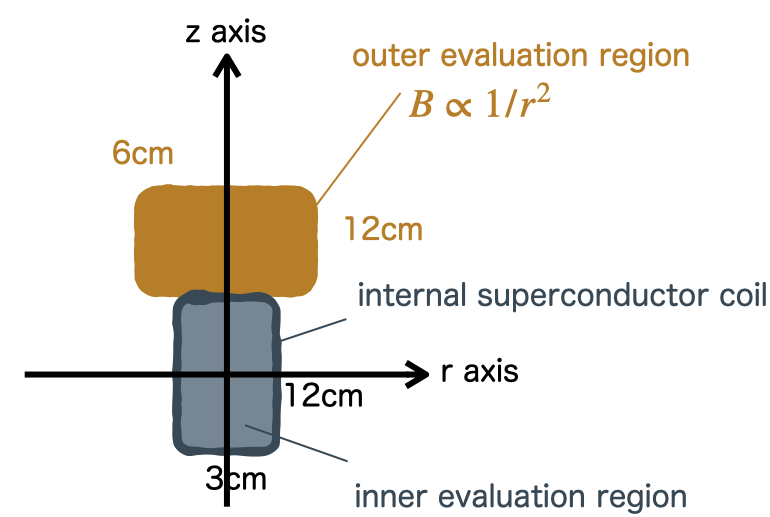
\includegraphics[width=18cm, bb=9 9 900 610]{./section4Optimal/evaluationRegion.png}
  \caption{Outer and inner field evaluation region.}
  \label{fig:evaluationRegion}
\end{figure}

This problem can be classified into the {\sl discrete nonlinear} optimization problem,
since the loss function is nonlinear to the variable $\mathbf{x}$ and
the turn position is limited to the fix tape width, which makes $\mathbf{x}$ to take discrete values.
Due to the solution space being discrete, we don't have many choices to solve it.
Among which includes the dynamic programming, the greedy method, the genetic algorithm and the modern machine learning methods like the reinceforcement learning, etc.
Here, to reach a comparatively general solution with limited calculation resource,
we have chosen the genetic algorithm which is able to explain the problem straight forward.
The detail is shown in the Method section.


\subsubsection{Method}
Within our calculation models, positions and fields are all calculated in 2D axisymmetric cylindrical coordinates $(r, z)$.
For instance, Fig. \ref{fig:coilDistributionSolenoid} shows a 2 layered solenoid windings,
with 30 turns per layer, 60 turns totally.
Note that since the length of the internal coil is 12 cm and the width of superconductor tape is 4 mm,
as shown in Tab. \ref{tab:optimizationOfCoilSpecification},
this is one of the simplest windings to fill up the whole length of the coil winding frame.
\begin{figure}[H]
  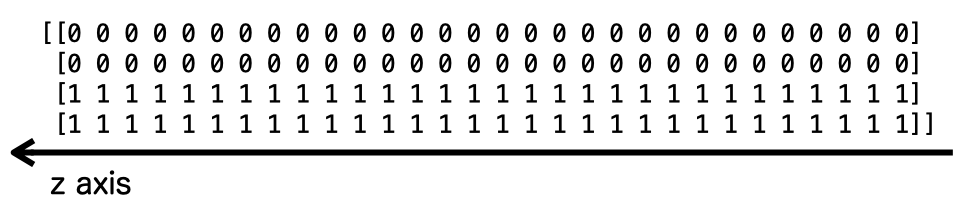
\includegraphics[width=18cm, bb=9 9 900 200]{./section4Optimal/solenoidCoilDistribution.png}
  \caption{Distribution of a solenoid windings.}
  \label{fig:coilDistributionSolenoid}
\end{figure}
For convenience, we named the axis parallel to the z axis "layer", the axis vertical to the z axis "stair".
In Fig. \ref{fig:coilDistributionSolenoid}, the windings have 2 layers and 30 stairs.

Next, we denote the method to produce next generation,
which we name "boom babies".
From any mother coil, we randomly choose 1 stairs to "grow" or "shrink".
The action "grow" means to stack one more turn on the specific stair,
while the action "shrink" means to remove one turn from the specific stair.
The maximum layer amount is set to be 4 for manufactoring reason,
and the minimum layer amount is zero.
Whether the selected stair should grow or shrink is also randomly chosen.
This action produces a "baby" coil from the "mother" coil.
Fig. \ref{fig:exampleDistribution} shows an example where the th stair is shrinked.
\begin{figure}[H]
  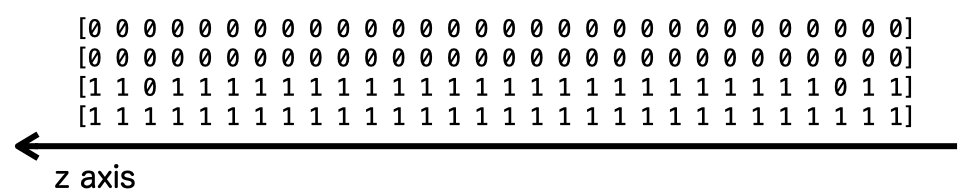
\includegraphics[width=18cm, bb=9 9 900 200]{./section4Optimal/exampleShrinkedCoil.png}
  \caption{Distribution of the coil shrinked from a 2 layered solenoid windigns.}
  \label{fig:exampleDistribution}
\end{figure}

The amount of individuals (coils) which can exist in each generation is set to 20.
For the begining of the calculation, we start with a normal 2 layered solenoid windings shown in Fig. \ref{fig:coilDistributionSolenoid}.
Since we only have 1 coil in the first generation, we boom 20 babies from this mother coil.
From the second generation, each coil booms 3 babies, results in all $20\times4 = 80$ (including mothor coils themself) coils.
From the 80 coils, we calculate their loss function and take the minimum 20 coils as survived individuals in the generation,
with the other 60 coils abandomed.
This is considered one step of the genetic algorithm.
When the average losses in the generation doesn't improve from the previous one,
we stop the calculation and take the least loss coil as the best solution.
The flow diagram of the program is shown in Fig. \ref{fig:flowOfGenetic}.
For the calculation of $B$ fields, the finite element method provided by commercial CAE software Comsol Multiphysics Inc. is used.
\begin{figure}[H]
  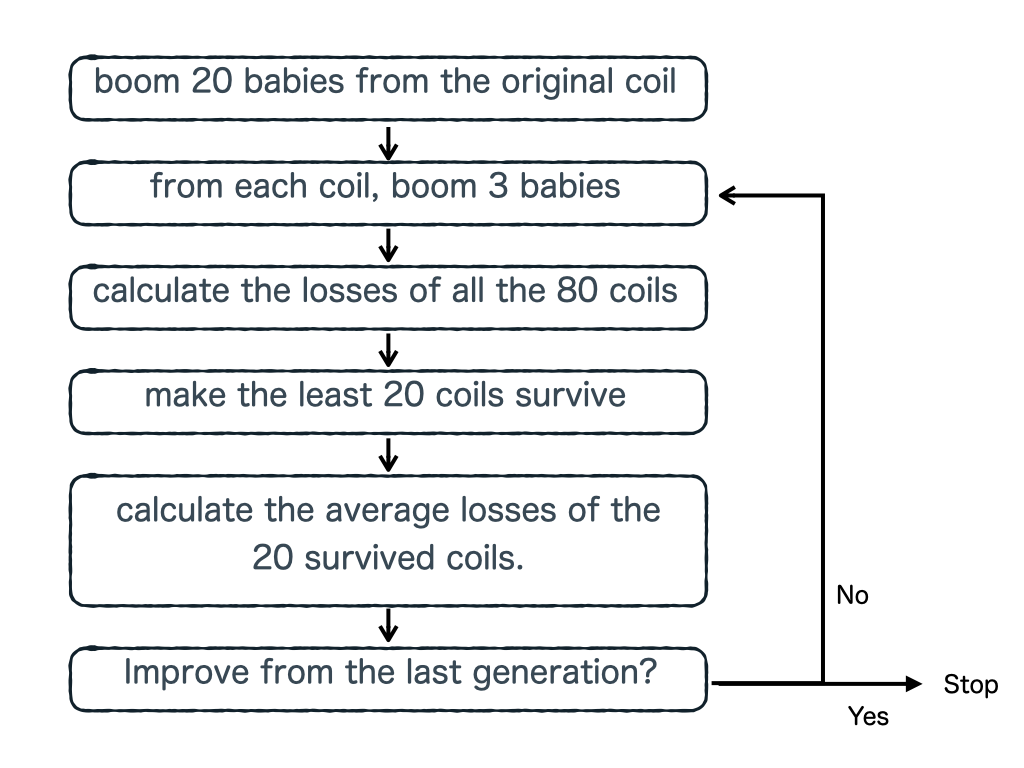
\includegraphics[width=18cm, bb=9 9 900 800]{./section4Optimal/geneticFlow.png}
  \caption{The flow of our genetic program.}
  \label{fig:flowOfGenetic}
\end{figure}

After the simulation, we have confirmed the result by an experiment.
Although the simluation has marked rectangular areas as evaluation region,
consider the accuracy of our equipment,
it is difficult ot measure the entire distribution in the evaluation resion.
Instead, we have taken the $B$ distribution along the z axis to represent the inner field,
and the $B$ distribution along the cross line on the top surface to represent the outer field.
The $B$ distribution on the both axises are measured and compared between the initial models and the optimized model.
Other details such as how the fields are measured are similar to the previous experiment,
and thus is ommited here.


\subsubsection{Result and Discussion}
The process of the optimization is shown in Fig. \ref{fig:optimizedCoilTrainingSteps},
and the initial solenoid coil and the ultimate optimized coil construction is shown in Fig. \ref{fig:optimizedCoilConstruction}.
\begin{figure}[H]
  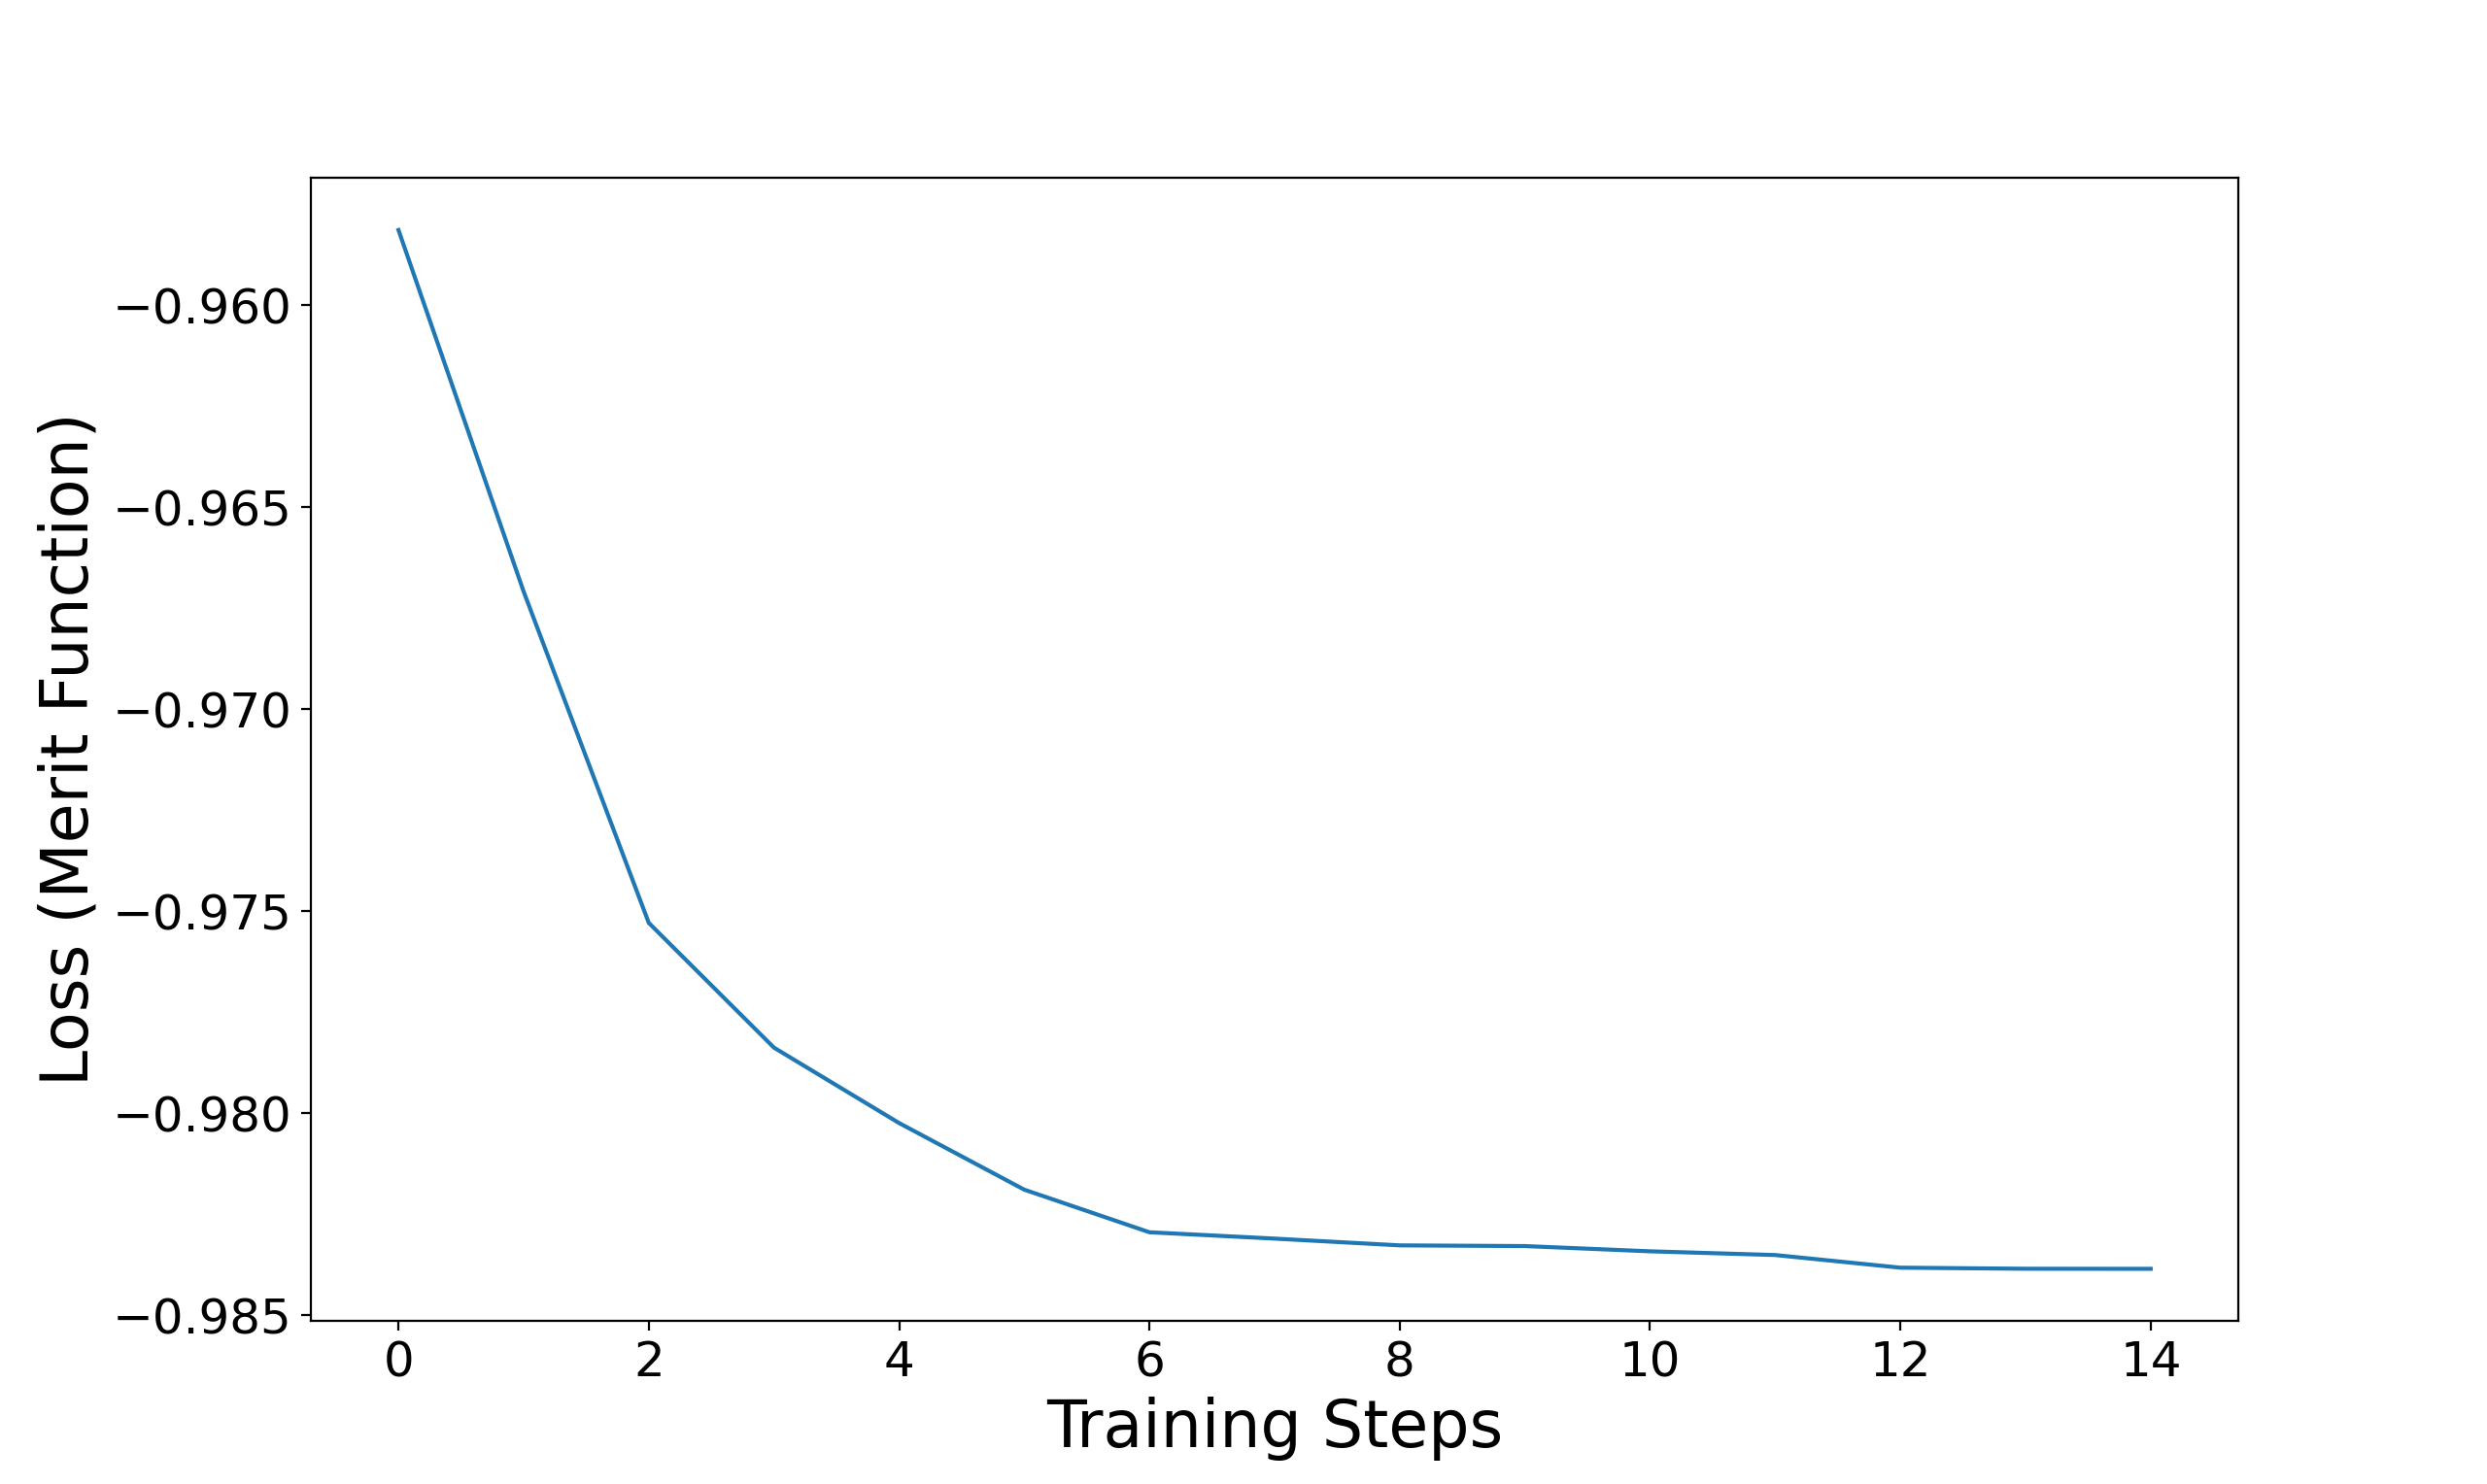
\includegraphics[width=18cm, bb=9 9 900 550]{./section4Optimal/averageLosses.png}
  \caption{Optimization process.}
  \label{fig:optimizedCoilTrainingSteps}
\end{figure}
\begin{figure}[H]
  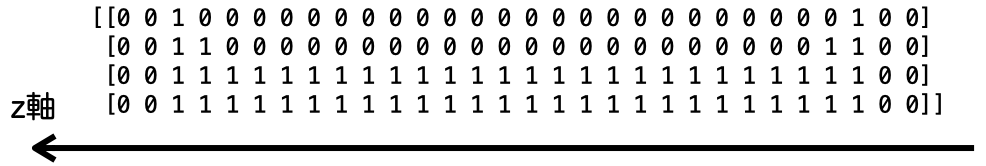
\includegraphics[width=18cm, bb=9 9 900 200]{./section4Optimal/optimizedCoilDistribution.png}
  \caption{Optimized coil distribution.}
  \label{fig:optimizedCoilConstruction}
\end{figure}
From Fig. \label{fig:optimizedCoilConstruction}, we can see that to achieve more cloaking ability,
more turns are needed near the edge and normal solenoid windings near the central part are just fine.
Also,

To confirm the calculation, we have manufacted the optimized coil and measured the shielding rates on the central axis and top cross line.
For comparison, the initial 2 layered solenoid coil are also manufacted and measured.
The experimental result along with the calculation are shown in Fig. \ref{fig:optimizedCoilExperimentResultCentral} and Fig. \ref{fig:optimizedCoilExperimentResultTopLine}.
\begin{figure}[H]
  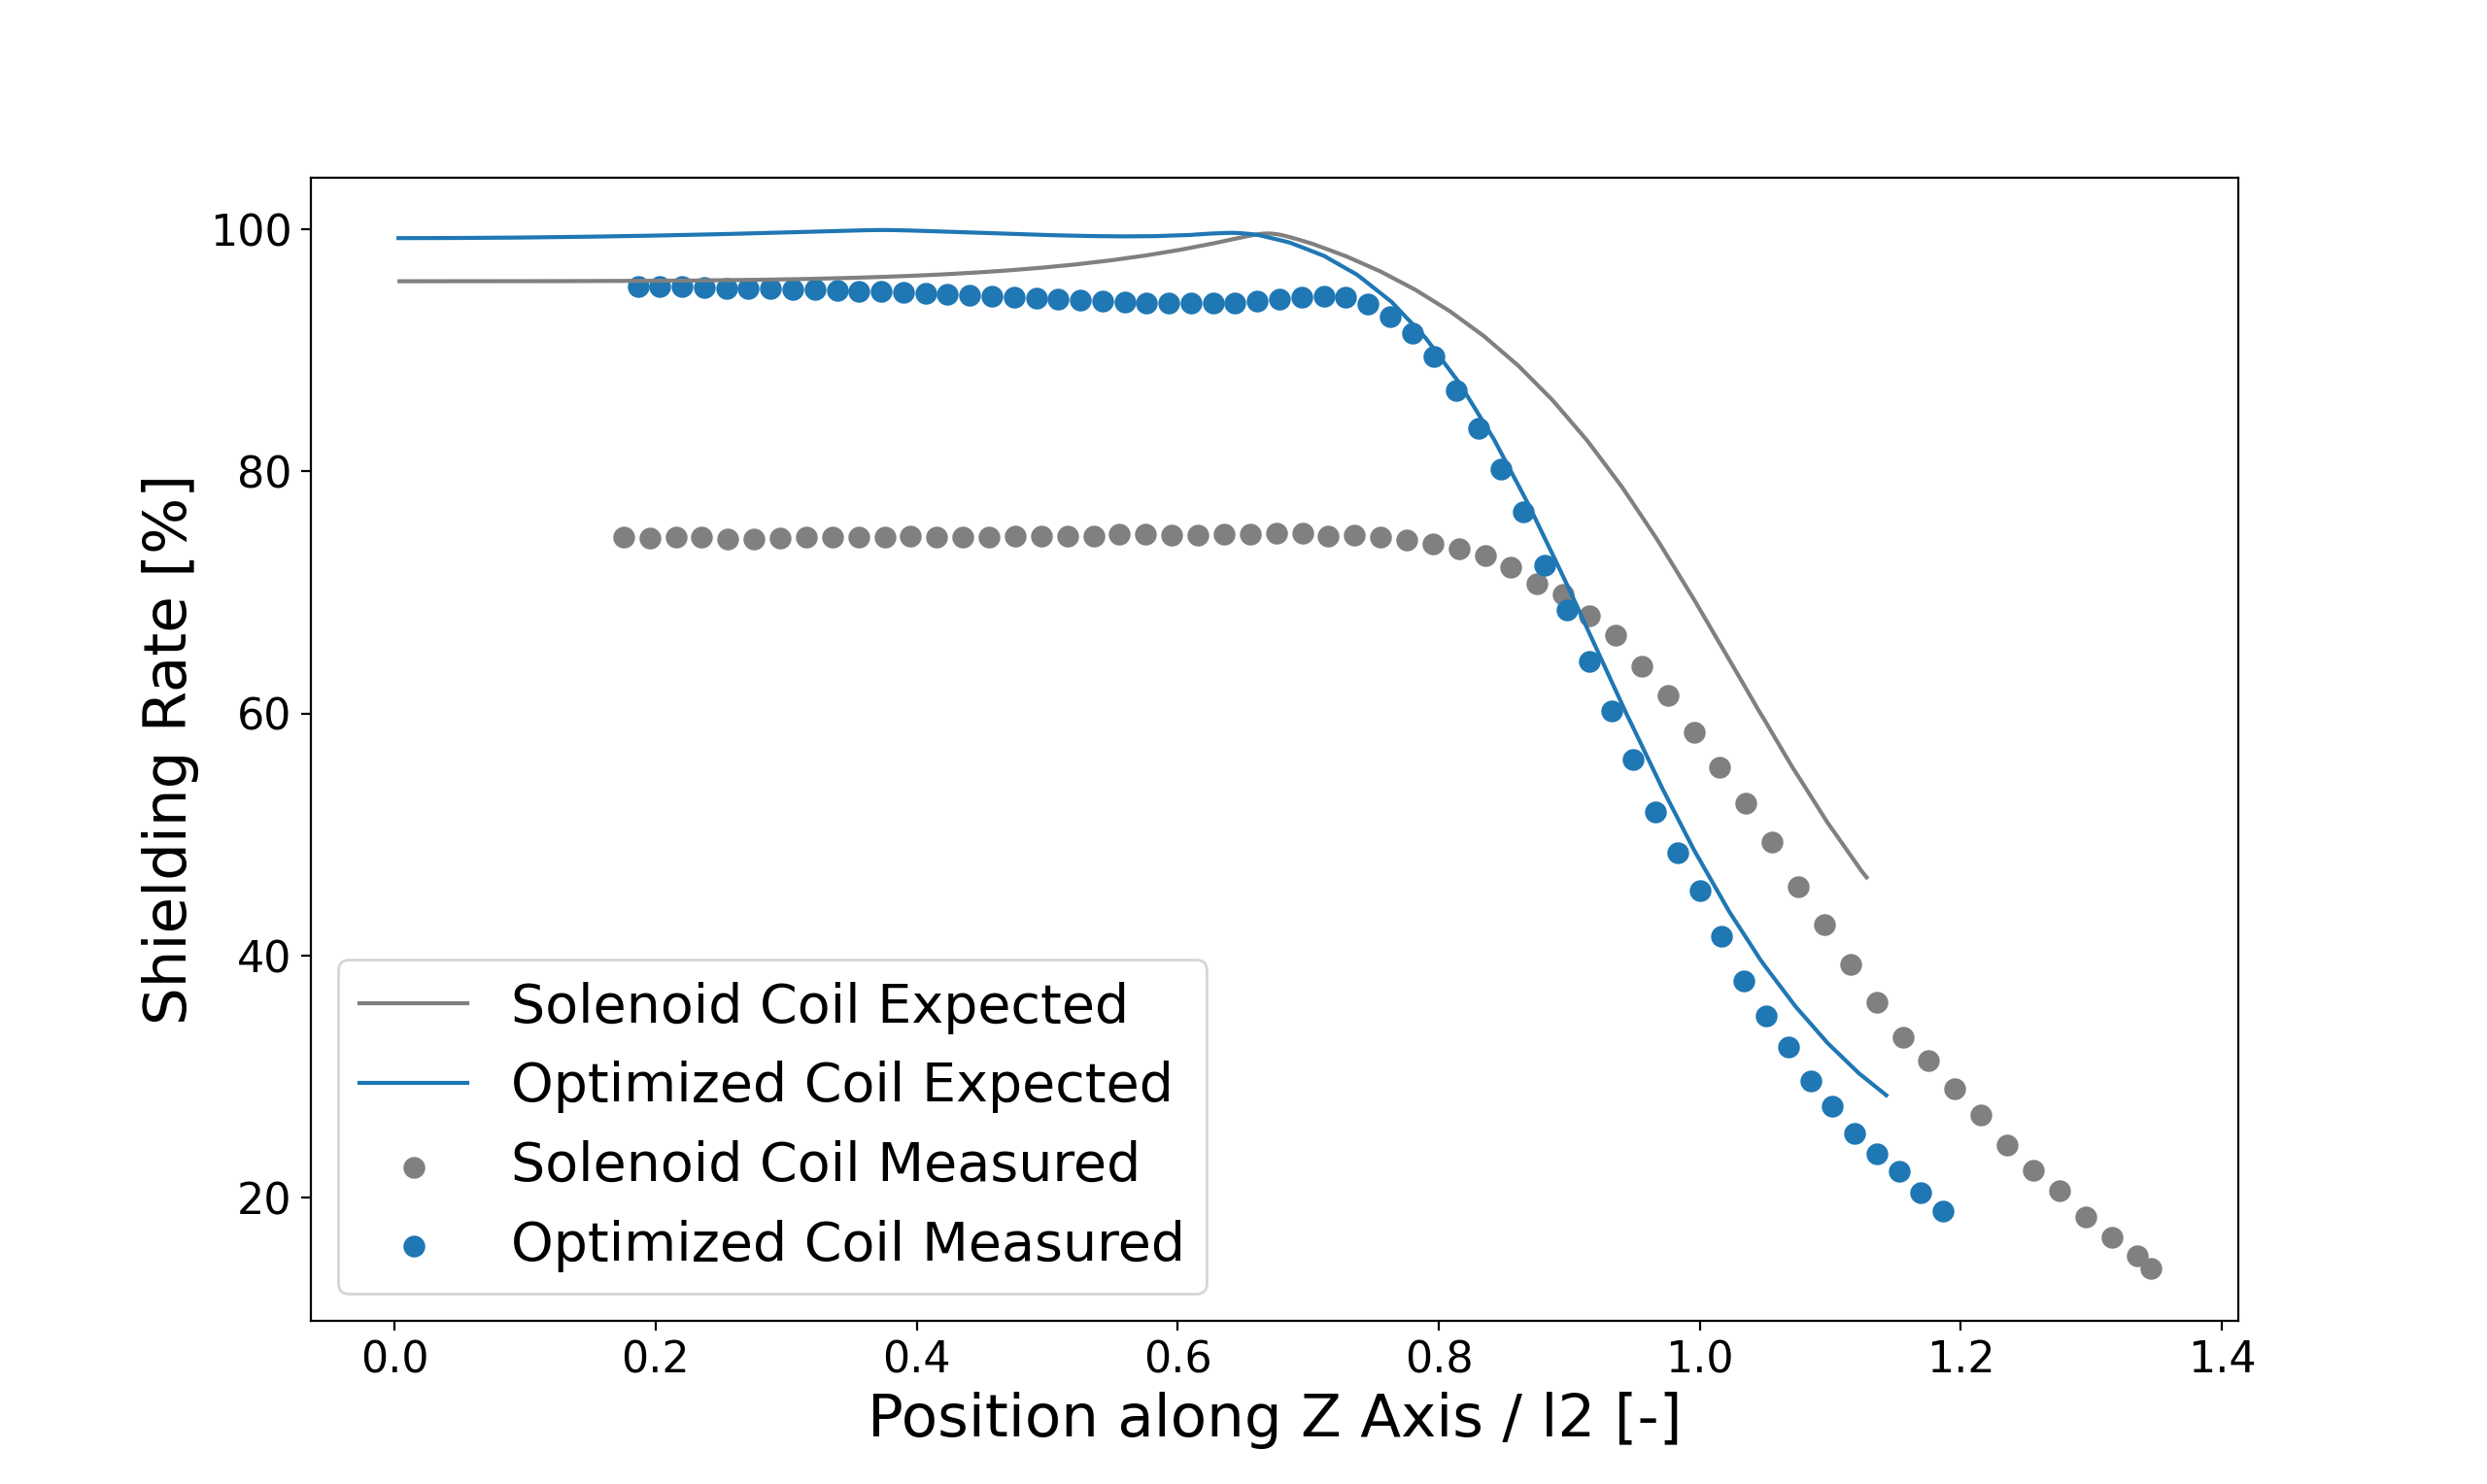
\includegraphics[width=18cm, bb=9 9 900 550]{./section4Optimal/combinedShieldingRates.png}
  \caption{Measured shielding rate along the central axis.}
  \label{fig:optimizedCoilExperimentResultCentral}
\end{figure}
\begin{figure}[H]
  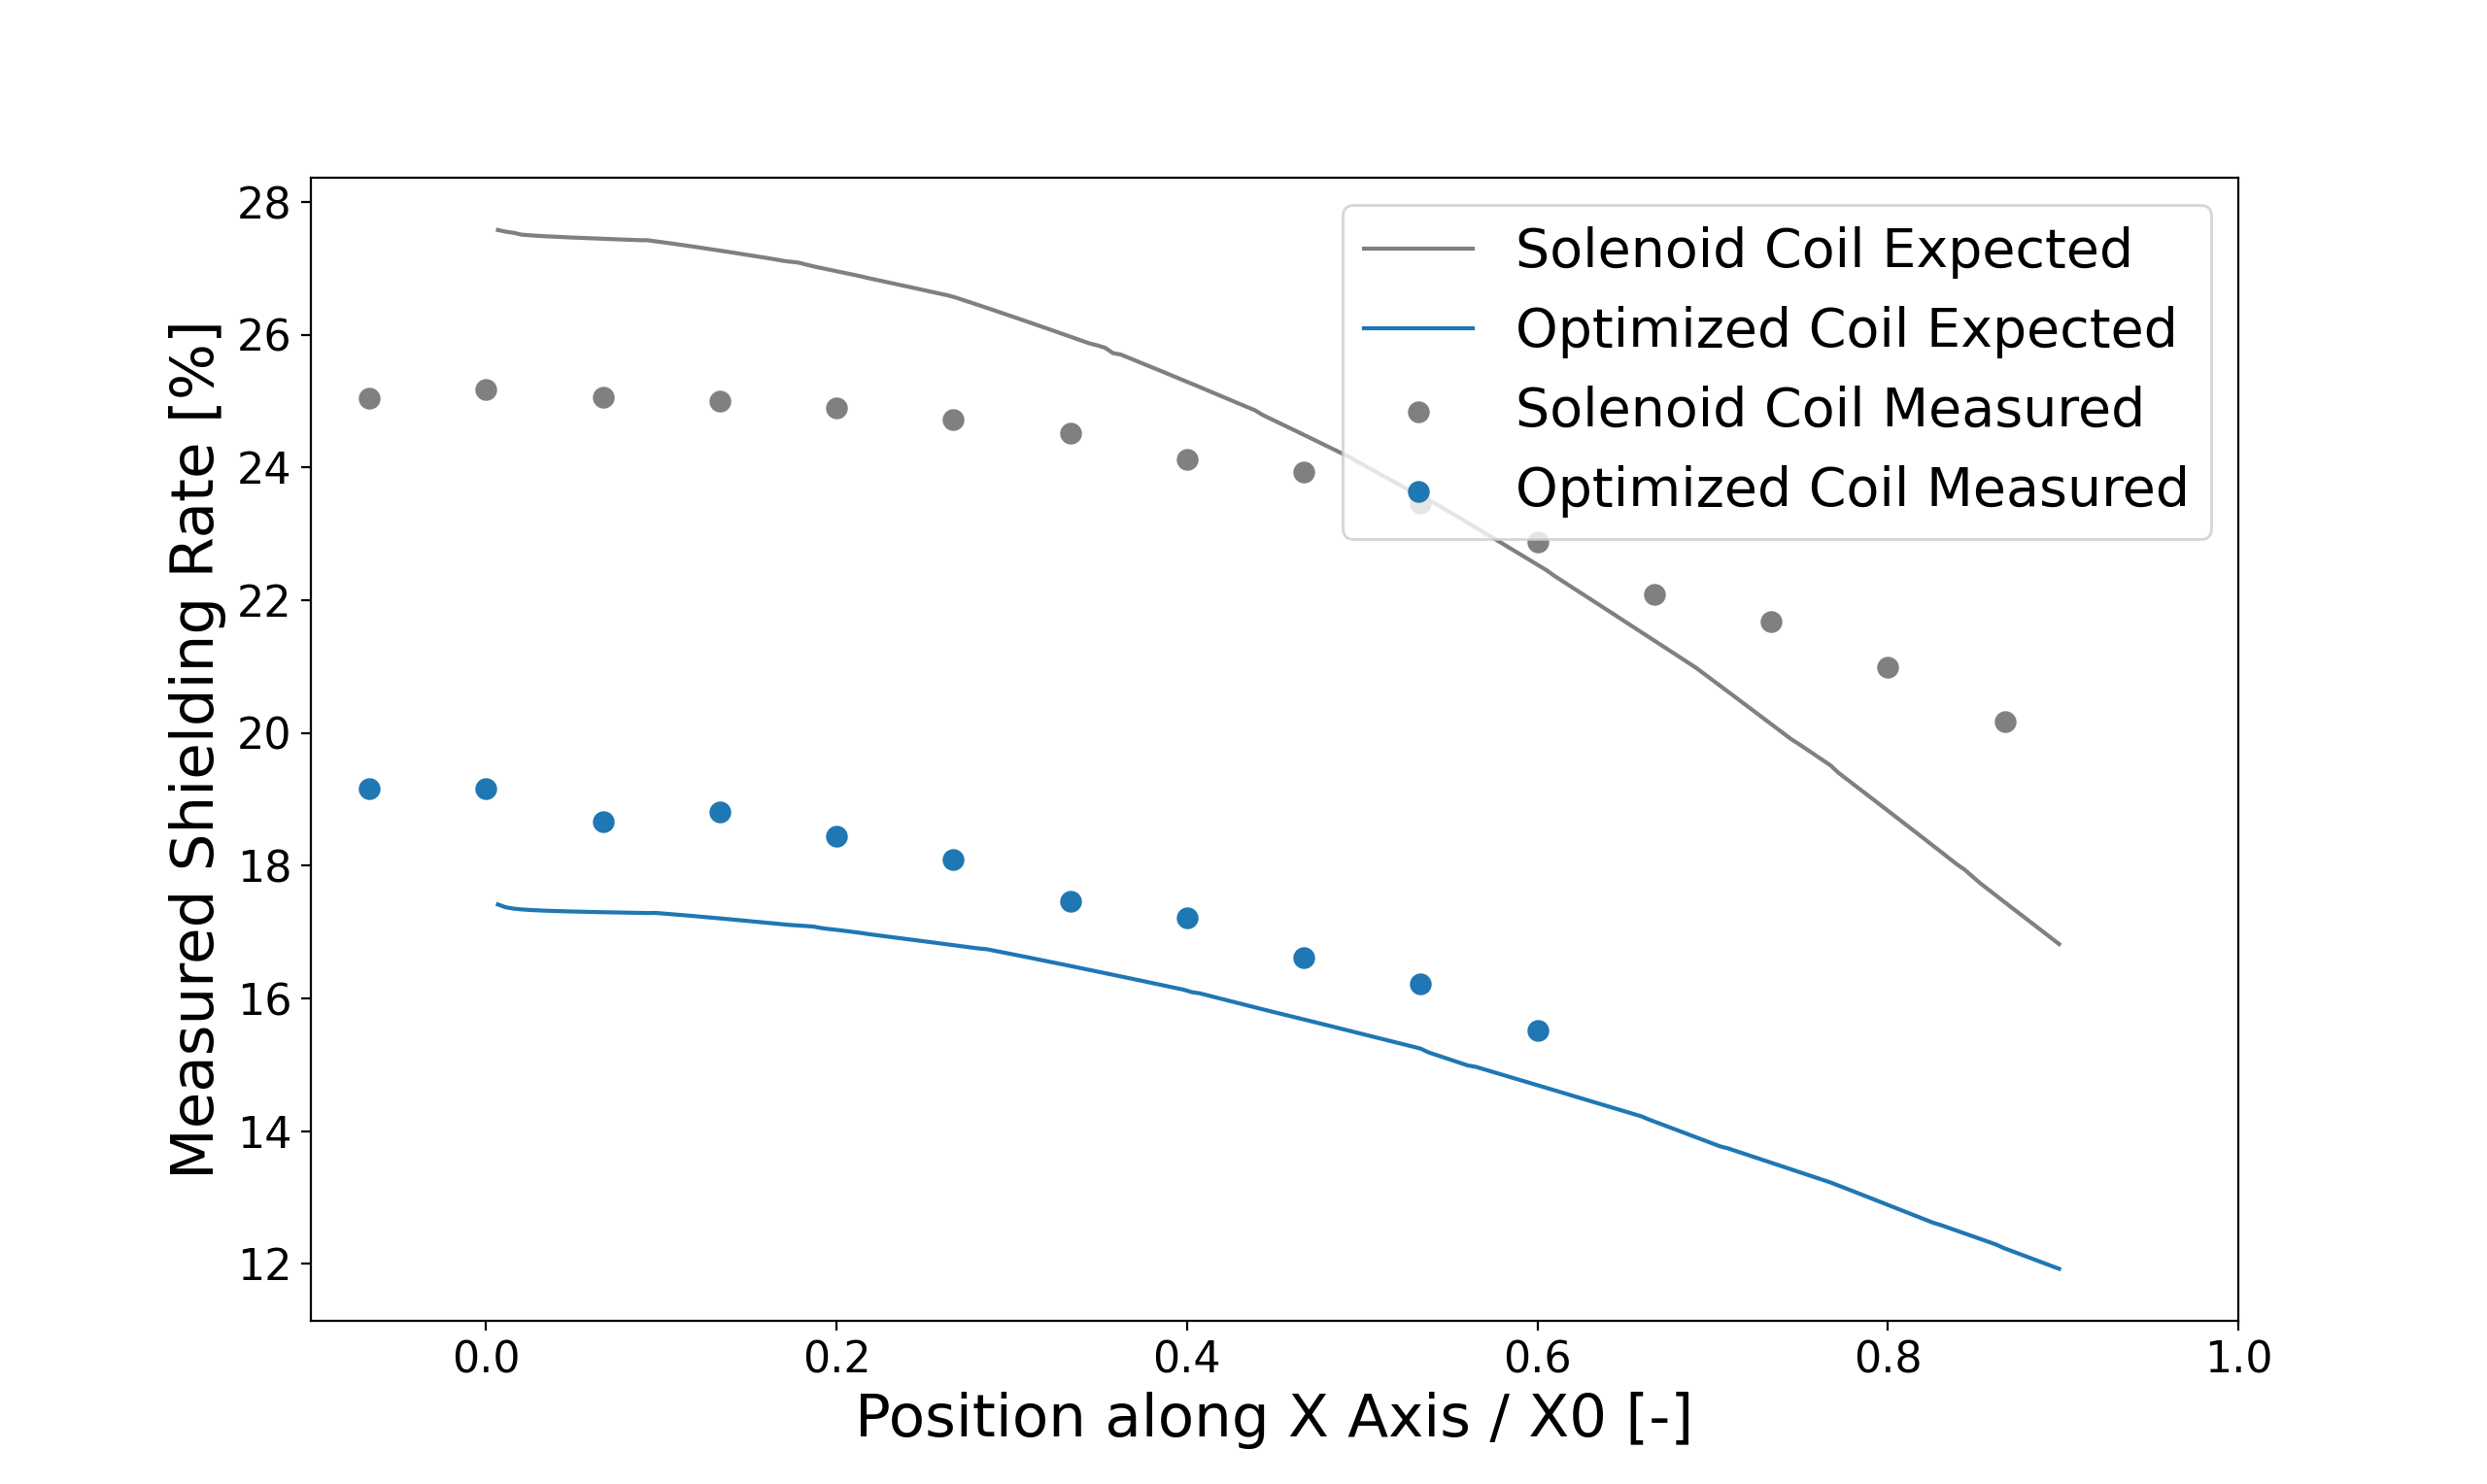
\includegraphics[width=18cm, bb=9 9 900 550]{./section4Optimal/combinedShieldingRatesTopLine.png}
  \caption{Measured shielding rate along the top line.}
  \label{fig:optimizedCoilExperimentResultTopLine}
\end{figure}
From Fig. \ref{fig:optimizedCoilExperimentResultCentral} we can see that for the inner field the optimized coil shows a better performance on shielding rates than the conventional solenoid,
and for the outer field the optimized coil the optimized coil reinforced the outer field.


\subsubsection{Conclusion}
In this section, we have show the result of our study on the optimized position a superconductor windings can be.
Through the simulation and experiment,
we have found that:
\begin{enumerate}
  \item Placing more turns near the edge increases the shielding rate, since the overshielding observed on a solenoid coil is released.
  \item Give the coil some margin on the edge reduces the disturbtion on the external field.
  This conclusion is considered reasonable due to the fact that $B$ field decays proportionally to $1r^2$.
\end{enumerate}


\subsection{Optimal Position of Ferromagnets}
In this section, we denote the optimal position of the ferromagnet.
As the above, the purpose, the theory, the method and finally the result would be denoted.


\subsubsection{Purpose}
The question about how to place the ferromagnet remains open.
The purpose of this section is to figure out figure out the best position of ferromagnets to achieve the best cloaking performance.


\subsubsection{Theory}
To translate the problem into mathmetical description,
we have first approximated the position of forromagnets by a four degree polynomial distribution function which denotes the corresponding $\rho$ components from the given $z$ components.
\begin{eqnarray}
  \rho_m(z_m|\mathbf{w}) = w_0 + w_1z_m + w_2z_m^2 + w_3z_m^3 + w_4z_m^4 + w_5z_m^5\\
  z_m \in \mathrm{[}0.5Z_0, 1.5Z_0\mathrm{]}\nonumber
\end{eqnarray}
where $Z_0$ represents the half length of the inner coil or the coil's top edge position,
$\rho_m$ represents the $\rho$ components of the ferromagnet,
$z_m$ represents the $z$ components of the ferromagnet,
$\mathbf{w}$ represents the weights of each term, which is the variable.
In this way, the optimization problem can be written in mathmetical form shown below.
\begin{eqnarray}
  \mathrm{variable}&:& \mathbf{w} = \{w_0, w_1, w_2, w_3, w_4, w_5\}\\
  \mathrm{loss\quad function}&:& f(\mathbf{w}) = mean\left(|\mathbf{B}_{in}(\mathbf{x})|\right) / mean\left(|\mathbf{B}_{out}(\mathbf{x})|\right)\\\nonumber
  \mathrm{constraint1}&:& g_1(\mathbf{w}) = \rho_m(\mathbf{w}|z_m=1.5Z_0) = -\left(w_0 + w_1(1.5Z_0) + ... + w_5(1.5Z_0)^5\right)\\\nonumber
  \mathrm{constraint2}&:& g_2(\mathbf{w}) = \rho_m(\mathbf{w}|z_m=0.5Z_0) = \left(w_0 + w_1(0.5Z_0) + ... + w_5(0.5Z_0)^5 \le \rho_0 \right) \le0\nonumber
\end{eqnarray}
The loss function can be anything which has minimum value when the inner field minimizes and the our field maximizes.
Constraints are aimed to limit the distribution function lies near the coil,
which guarantees the solution to have reasonable physical meaning.
The problem can be seen as a {\sl continuous constrained linear} optimization problem,
since the main variable $\mathbf{w}$ takes continuous values,
the polynomial is linear to $\mathbf{w}$.
This kind of optimization problem can be solved by the conventional method of Lagrange multiplier under Karush-Kuhn-Tucker(KKT) condition,
by introducing the Lagrange function:
\begin{eqnarray}
  Lagrange Function \nabla L(\mathbf{w, \lambda}) = \nabla\left( f(\mathbf{w})+\lambda_1 g_1(\mathbf{w})+\lambda_2 g_2(\mathbf{w})\right)=0
\end{eqnarray}
All left is to solve the simultaneous equations of the KKT condition.
\begin{eqnarray}
  \frac{\partial L}{\partial w_0}&=&\frac{\partial}{\partial w_0}f(\mathbf{w})+\lambda_1(-1)+\lambda_2(1)=0\\
  \frac{\partial L}{\partial w_1}&=&\frac{\partial}{\partial w_1}f(\mathbf{w})+\lambda_1(-1.5Z_0)+\lambda_2(0.5Z_0)=0\\\nonumber
  \frac{\partial L}{\partial w_2}&=&\frac{\partial}{\partial w_2}f(\mathbf{w})+\lambda_1(-(1.5Z_0)^2)+\lambda_2((0.5Z_0)^2)=0\\\nonumber
  &.&..\\\nonumber
  \frac{\partial L}{\partial \lambda_1}&=&g_1(\mathbf{w})=0\\\nonumber
  \frac{\partial L}{\partial \lambda_2}&=&g_2(\mathbf{w})=0\nonumber
\end{eqnarray}

However, this requests the first derivate of $f(\mathbf{w})$ which we don't have.
Therefore, we have used an iterative method to solve the equations, the schametic procedure is shown below.
\begin{eqnarray}
  w_0^{(k+1)} = w_0^{(k)} - \alpha\frac{\partial f(w^{(k)})}{\partial w_0}\\
  w_1^{(k+1)} = w_1^{(k)} - \alpha\frac{\partial f(w^{(k)})}{\partial w_1}\\\nonumber
  ...\\\nonumber
  w_5^{(k+1)} = w_5^{(k)} - \alpha\frac{\partial f(w^{(k)})}{\partial w_5}\nonumber
\end{eqnarray}
where the derivate part $\frac{\partial f(w^{(k)})}{\partial w_0}$ is substituded by numerical derivate.


\subsubsection{Method}
The optimization procedure is shown below
\begin{enumerate}
  \item Randomly choose $\mathbf{w}$, which defines the initial distribution of the ferromagnet.
  \item Calculate derivate of f $f(\mathbf{w+\pm \Delta})$.
  \item Update $\mathbf{w}$ to the direction minimizing $f$.
  \item Repeat until $\mathbf{w}$ is not improving.
\end{enumerate}
For the calculation of the inner and outer field,
finite element method is used.
To reduce the calculation time, we have neglect the nonlinear permeability generally seen in ferromagnet
and used a fix permeability of 100,
which is relatively small but is just fine to give us the strong magnetization under the current condition.
For the optimization algorithm, we have chosen the trust-constraint algorithm,
which belongs to the quasi-newton method of optimization.
The detail specification used in the calculation is shown in Fig. \ref{fig:FMEvaluationRegion} and Tab. \ref{tab:FMSpecification}.
\begin{figure}[H]
  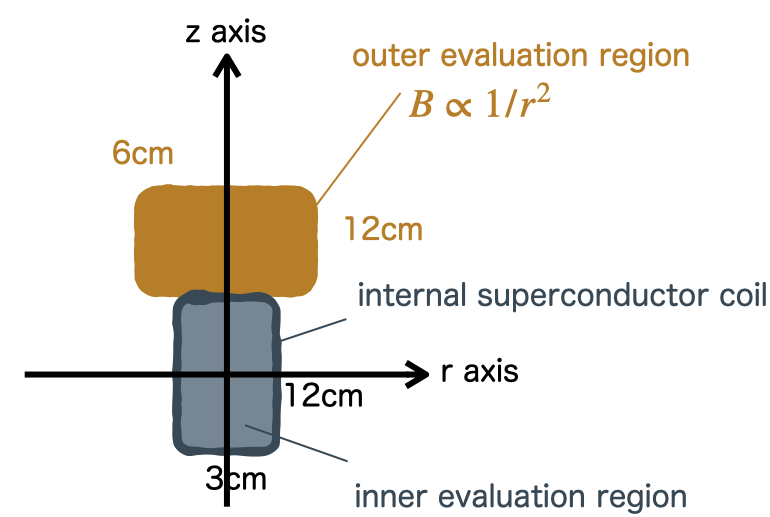
\includegraphics[width=18cm, bb=9 9 900 600]{./section4Optimal/evaluationRegion.png}
  \caption{Evaluation region.}
  \label{fig:FMEvaluationRegion}
\end{figure}
\begin{table}[H]
  \centering
  \caption{Specification of the ferromagnet optimization.}
  \label{tab:FMSpecification}
  \begin{tabular}{cc}\hline\hline
    Thickness of Ferromagnet & 1 [mm]\\
    Relative Permeability & 100 (fix)\\
    Loss Function & average inner field / average outer field\\\hline\hline
  \end{tabular}
\end{table}


\subsubsection{Result and Discussion}
The result of the optimization progress is shown in Fig. \ref{fig:FMOptimization}.
\begin{figure}[H]
  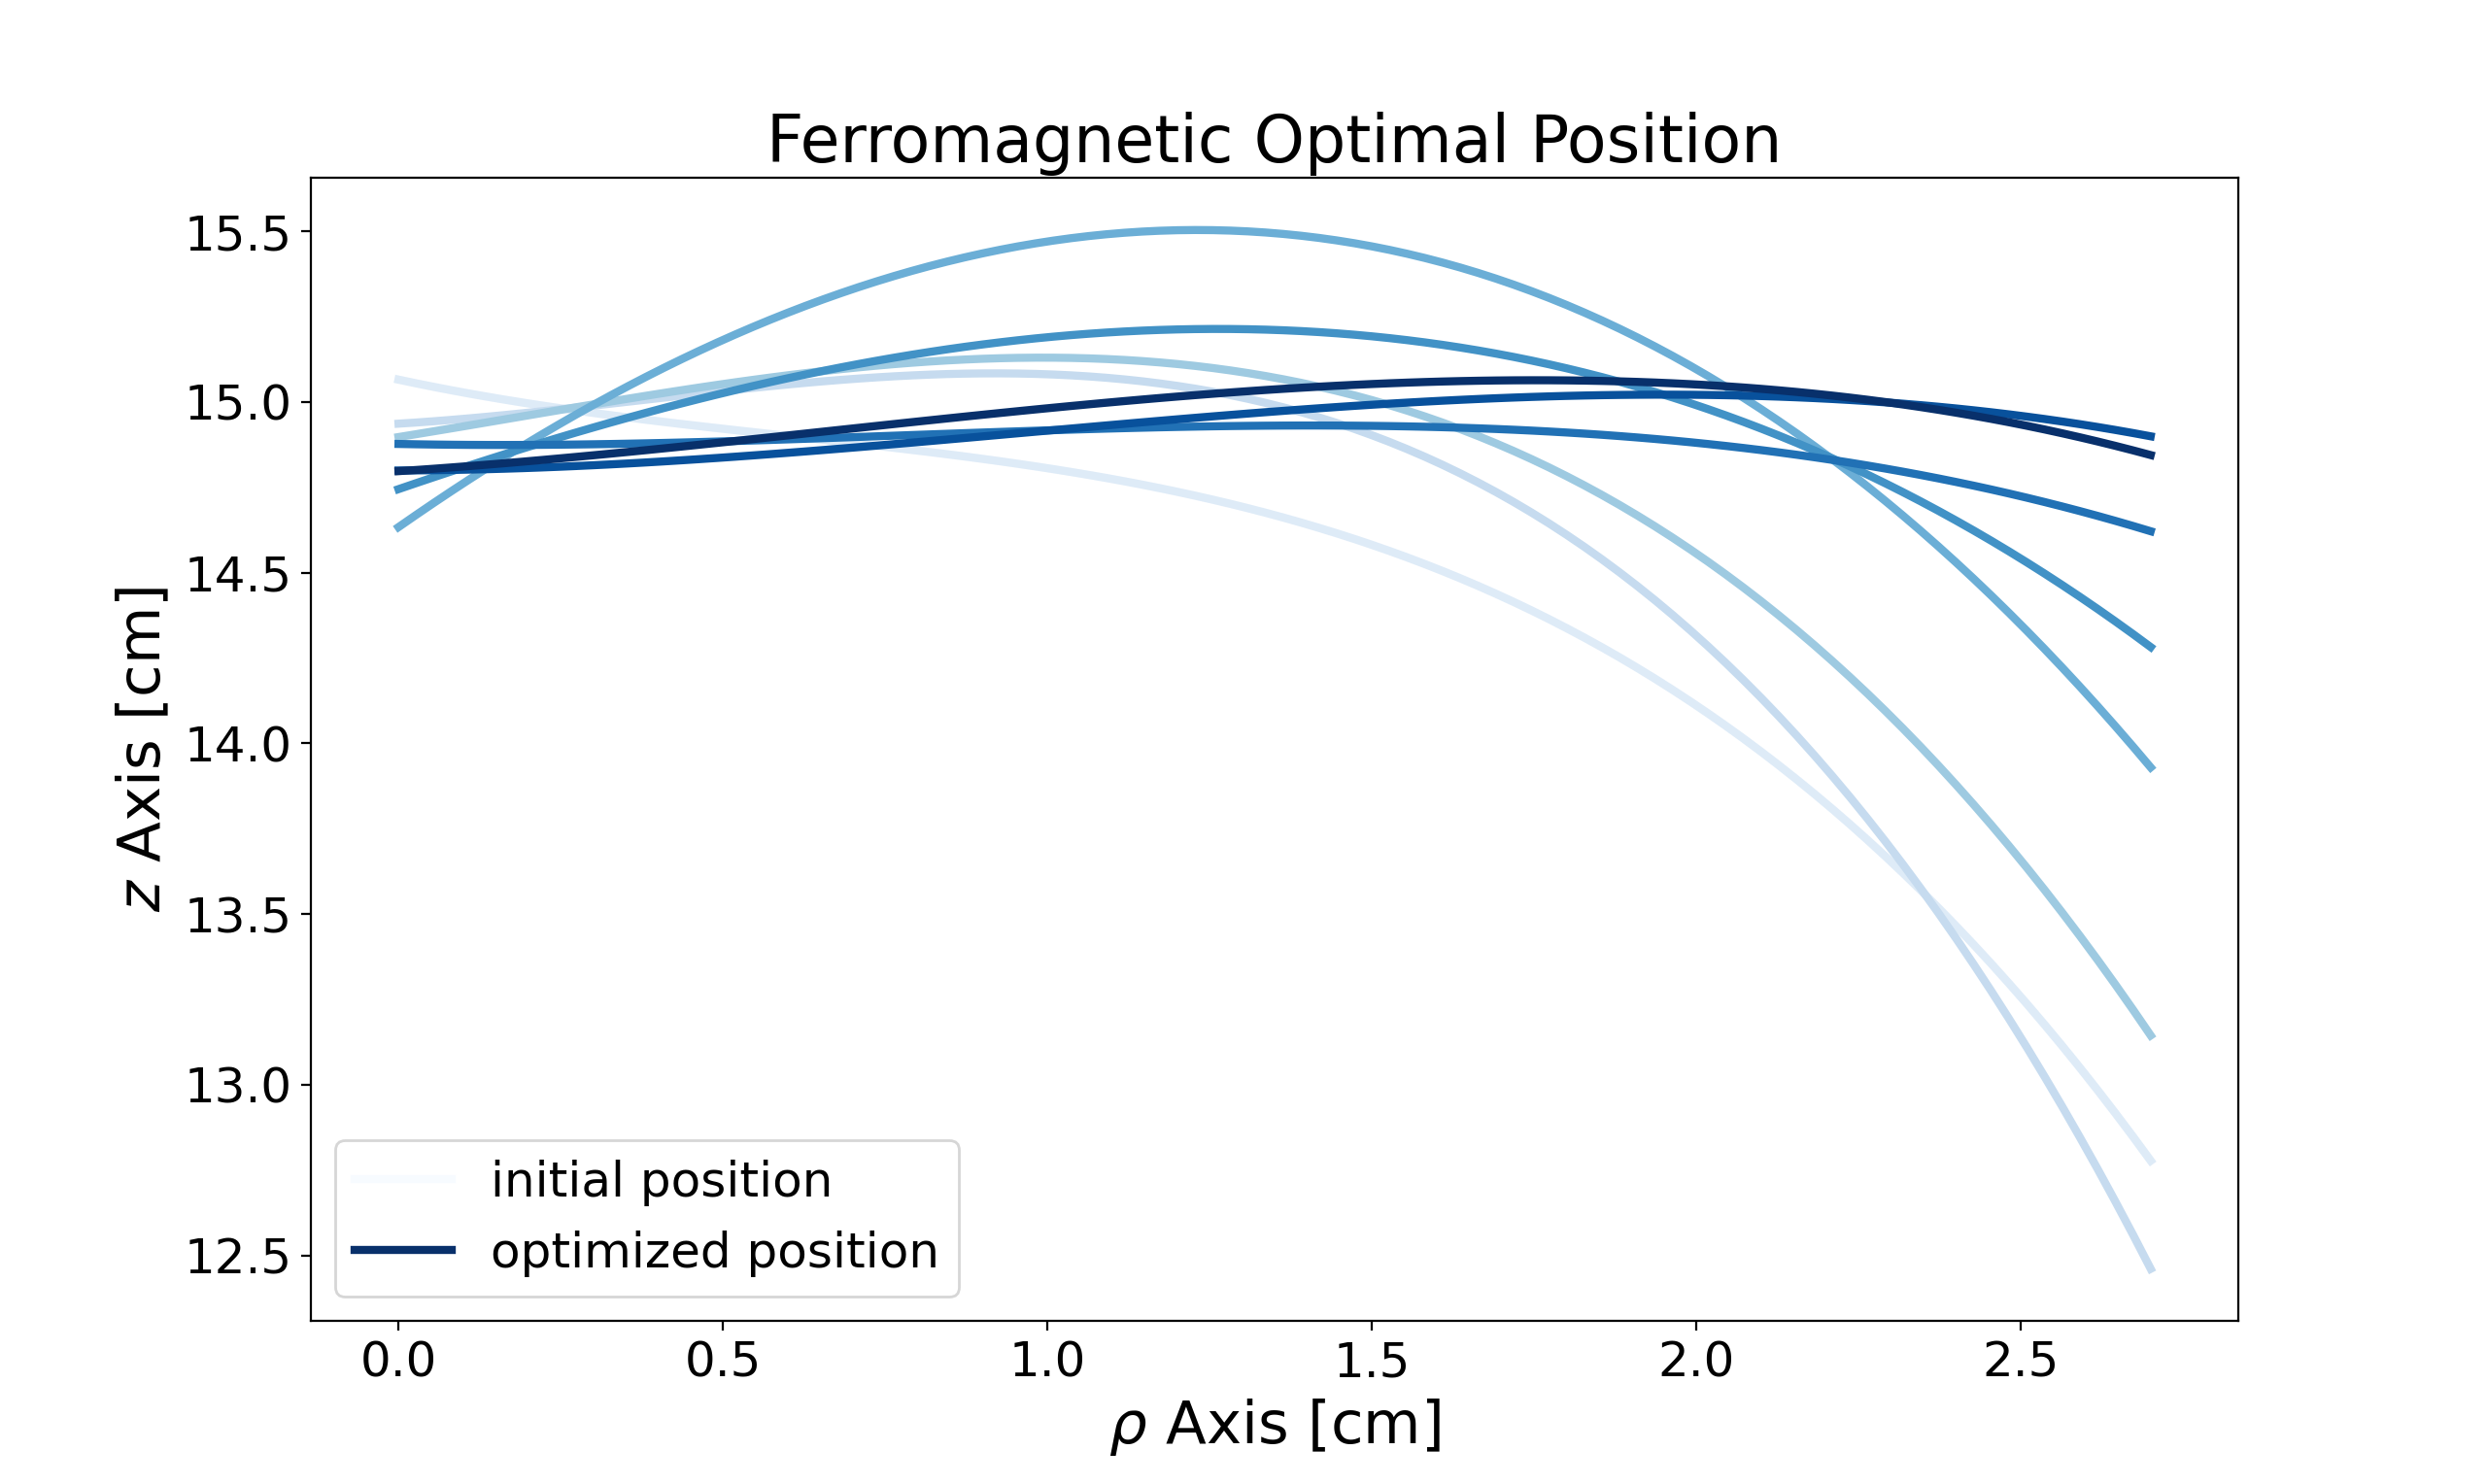
\includegraphics[width=18cm, bb=9 9 900 550]{./section4Optimal/FMOptimization.png}
  \caption{Optimization progress.}
  \label{fig:FMOptimization}
\end{figure}
In Fig. \ref{fig:FMOptimization}, the optimization have started from the lightest line, then the darker,
finally the darkest line which lies almost flat on the edge of the internal coil.
The result indicates that the best position of the ferromagnet to be placed is about flat on the edge.

To confirm this result, the magnetic field distribution near the coil is shown below,
with the comparison of whether the ferromagnet is included.
\begin{figure}[H]
  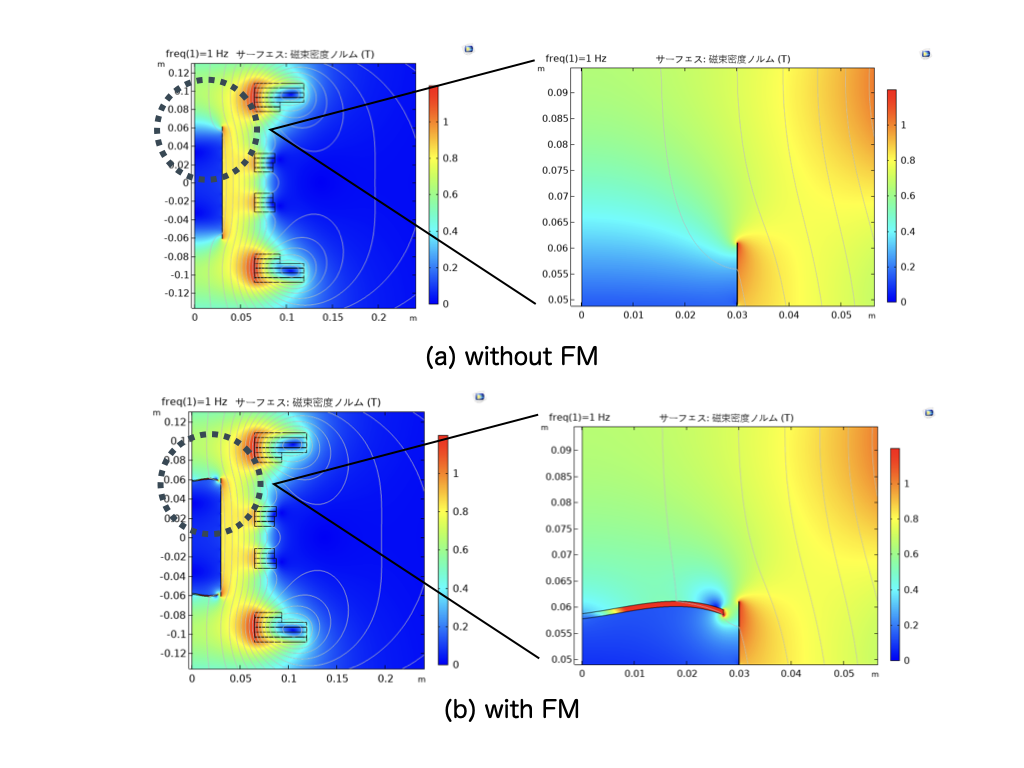
\includegraphics[width=18cm, bb=9 9 900 550]{./section4Optimal/FMDistribution.png}
  \caption{The $B$ field distribution in situations (a) without ferromagnet (b) with ferromagnet.}
  \label{fig:FMDistribution}
\end{figure}
\begin{figure}[H]
  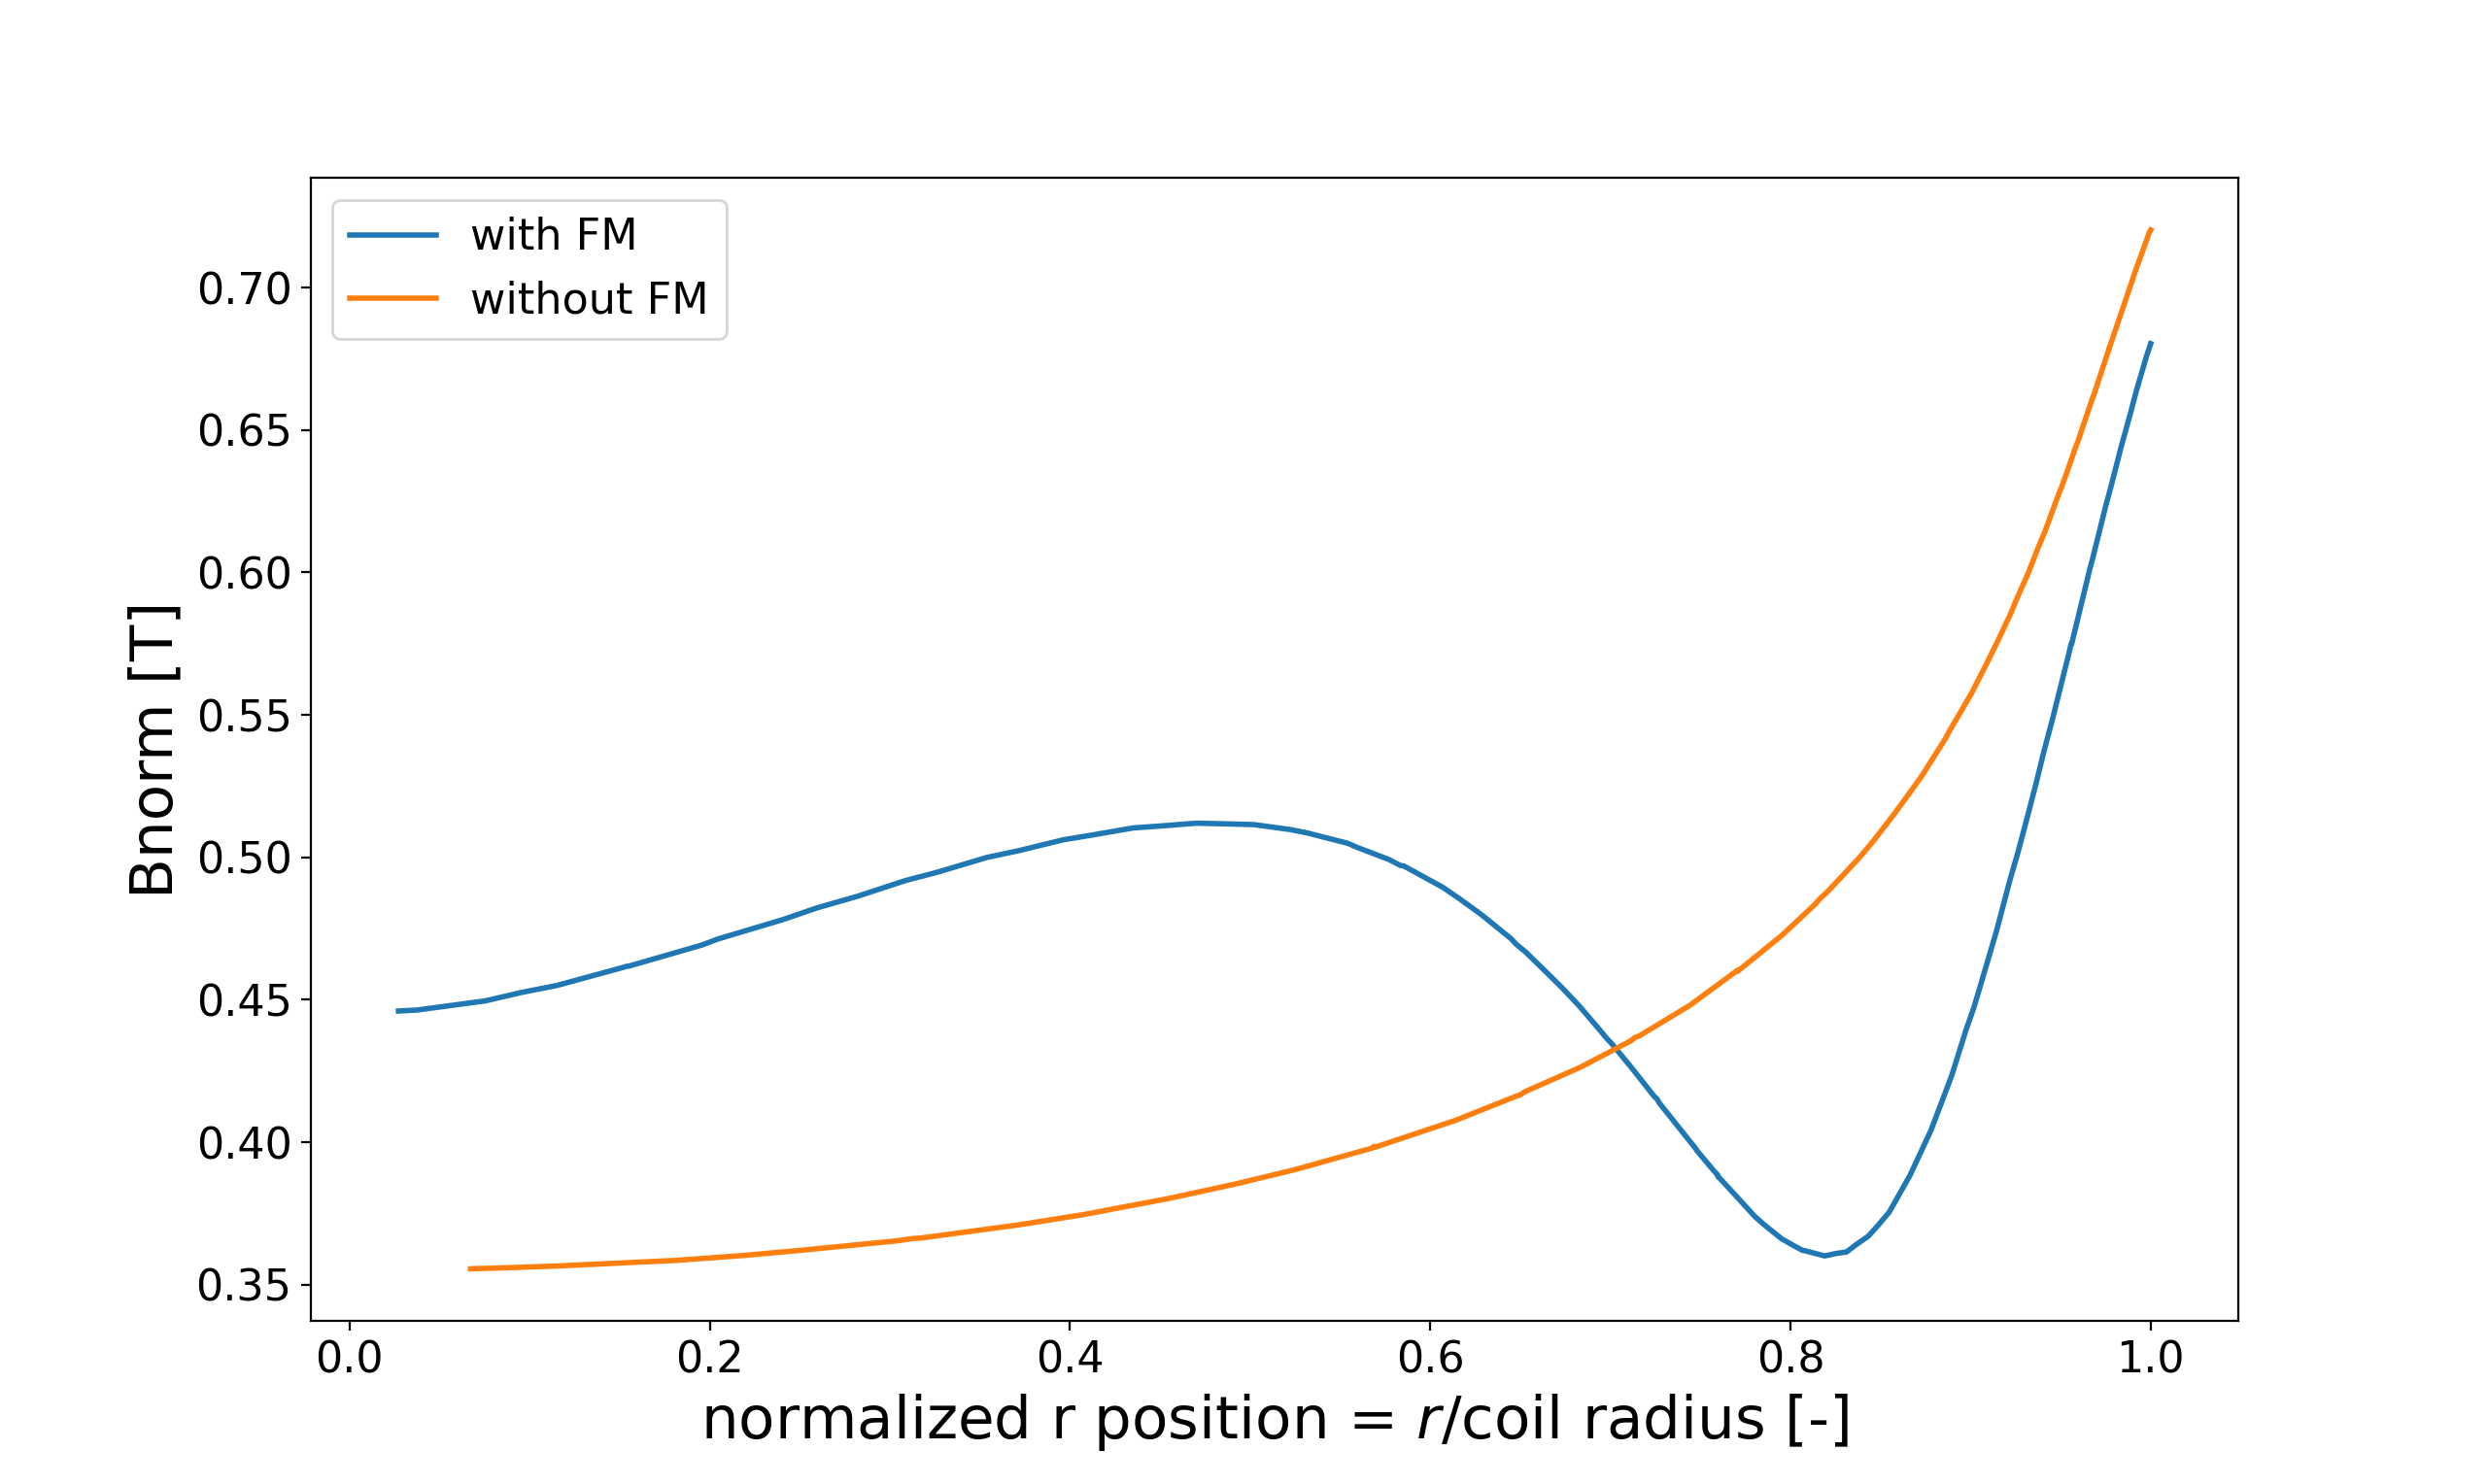
\includegraphics[width=18cm, bb=9 9 900 550]{./section4Optimal/FMDistributionTopLine.png}
  \caption{The $B$ field distribution on top line.}
  \label{fig:FMDistribution}
\end{figure}
From \ref{fig:FMDistribution} we can find that the external field distribution around the top edge of the inner coil is reinceforced when the ferromagnet is placed on the optimized position.
Also, if we look into the field on the ferromagnet carefully,
one can find that the ferromagnet is generating field over 1 T,
which is considered impossible in practice.
This results from the neglection of the nonlinear permeability of the ferromagnet.
Ferromagnets usually have maximum magnetization around 700 mT.
Instead of taking this limitation into consideration, which would have a bad impact on the convergence,
we approach it using a fix permeability,
which is a linear model thus can generate magnetization over the expected.
This may seem a bad idea, but since we are facing a condition that
the ferromagnet being placed under a very strong field of several Tesla exceeding the maximum magnetization,
the optimized result in our simulation can be explained as the best position at which the ferromagnet performs its maximum magnetization.
Therefore, this result is considered correct in strong fields.

However, this result has also exposed the problem of our proposed Electromagnetic Induction Type Magnetic Cloak,
which is,
the cloaking ability relying on the maximum magnetization of the ferromagnet.
Since this model uses ferromagnet to compensate the outer field near the coil edge,
the maximum fields it can generate is determined by the maximum magnetization of the ferromagnet.
For instance, a magnet having maximum 700 mT magnetization cannot compensate more than about 10\% of the outer field when it is imposed by 10 T magnetic field.
In our case of the spaceuseage, only a 2 T field is needed so that the proposal should be appliable,
but when it comes to other case in which 10 T or 20 T shielding is requested,
the cloaking ability cannot be achieved.
Of course, even in the cases with imposed field above 10 T, a satisfying shielding ability can be expected since the superconductor should work problemlessly.


\subsubsection{Conclusion}
In this chapter,
we have denoted the optimized position of placing the ferromagnet such that the inner field can be minimized and the outer field can be maximized.
After our calculation, the best position is found to be almost flat on the edge,
which have the scalability to much more field.
Howver, the provided magnetization is limited by the maximum magnetization the ferromagnet can provide,
which is mostly up to 700 mT.


\newpage
\begin{thebibliography}{20}
  \bibitem{2_1} Dirk P. Kroese, "Handbook of Monte Carlo Methods", Wiley Series in Probability and Statistics (2014)
\end{thebibliography}
